%!TEX root = ../diploma.tex

\section{Результаты экспериментов}\label{sec:exp}

\begin{figure}
\centering
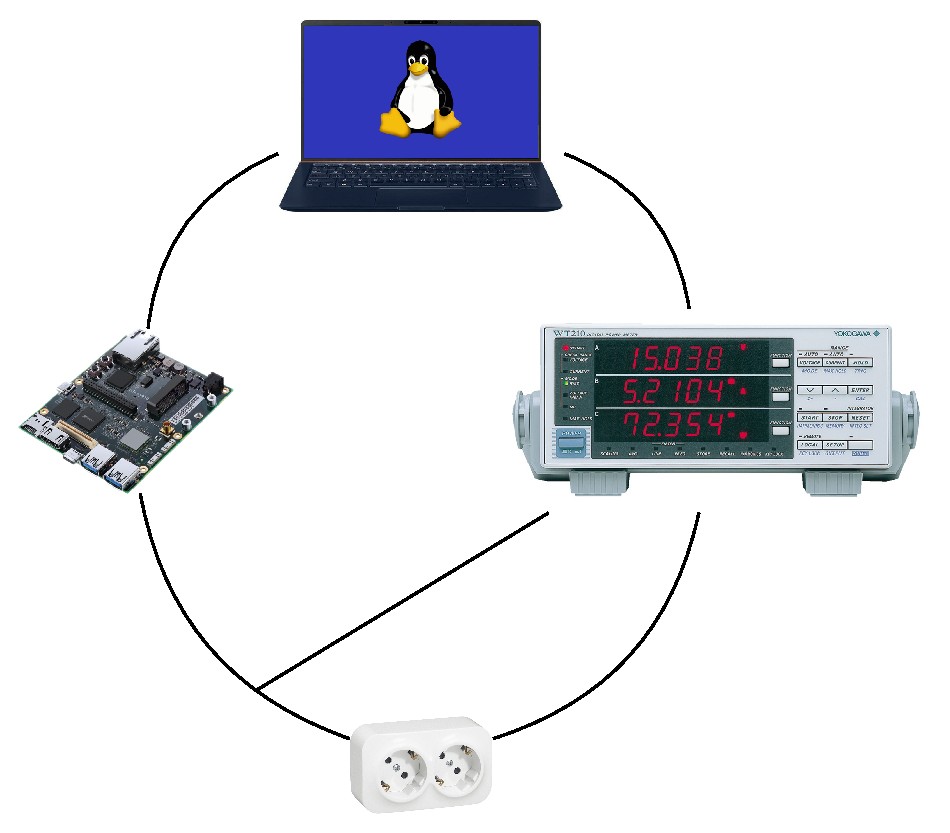
\includegraphics[scale=0.8]{setup}
\caption{Экспериментальная установка}
\label{fig:setup}
\end{figure}

В таблице~\ref{tab:exps} приведены полученные результаты замеров времени и
памяти для некоторых моделей НС: ResNeXt~\cite{resnext},
GoogLeNet~\cite{googlenet}, MobileNetV2~\cite{mobilenetv2},
Xception~\cite{xception}, InceptionV3~\cite{inceptionv3}. При конфигурации
предложенного метода количество групп выбрано одинаковым для всех слоев и
равняется либо 1, либо 2 (поскольку для всех сетей, кроме ResNeXt, размеры
получаемых слоев не превосходят четырех вершин). Из этой таблицы видно, что для
всех НС, кроме ResNeXt, оптимальное потребление памяти (по сравнению с
изначальной эвристикой оптимизации памяти) достигается уже при одной группе, и
разбиение на две группы также не дает улучшения по времени исполнения.

Представляет интерес более тщательный анализ экспериментов для ResNeXt (СНС с
групповыми свертками размера 32). На Рис.~\ref{fig:exp_dispatch_groups}
приведены полученные значения времени исполнения, объема используемой памяти,
числа циклов ожидания обращений в память ГП и среднее потребление электрической
энергии на запуск НС без учета потребления в покое. Оптимальный выбор числа
групп может быть нетривиален: например, исходя исключительно из времени
исполнения, будет оптимально разбить каждый слой на две группы. Если взять также
в расчет потребление памяти и электрической энергии, наилучшим значением может
оказаться 16 или 8 групп. При разбиении на две группы ускорение составляет
6.85\%, а потребление памяти сокращается на 72.4\%.

Полученное сокращение времени вычислений при увеличении числа групп говорит о
том, что модель~\ref{eqn:speedup} оказывается слишком упрощенной. А именно, она
не учитывает, каким образом организован доступ в память ГП ее вычислительными
ядрами. В нашем случае разбиение ResNeXt на две группы вместо одной дает
относительное ускорение на 3.65\%, также сокращается потребление памяти на
2.68\%.

Приведенные измерения производились на плате HiKey970 с мобильным графическим
процессором ARM Mali-G72 MP12, интегрированном в систему на кристалле HiSilicon
Kirin 970. Реализация всех методов и экспериментов произведена в
программно-аппаратной части библиотеки искусственного интеллекта MindSpore Lite
с использованием языка C++ и интерфейса прикладного программирования Vulkan.
Показатели ГП устройства были получены профилированием набором инструментов Arm
Development Studio. Потребление электрической энергии было посчитано при помощи
цифрового измерителя мощности Yokogawa WT210, показания с которого считывались
утилитой командной строки Yokotool\footnote{Исходный код \texttt{Yokotool}:
\url{https://github.com/intel/yoko-tool}.}. Визуально используемая
экспериментальная установка изображена на Рис.~\ref{fig:setup}.

\tabulinesep = 4pt

\begin{table}
    \caption{Результаты экспериментов}
    \label{tab:exps}
    \begin{tabu} to \textwidth{ X[1.6,l] X[1.45,l] *{5}{X[c]}}
        \hline
        Алгоритм & & \tiny{ResNeXt} & \tiny{GoogLeNet} & \tiny{MobileNetV2} &
        \tiny{Xception} & \tiny{InceptionV3}\\
        \thickhline
        \multirow{2}{3cm}{Базовая реализация} & время, мс & 234 ± 5 & 80 ± 3 & 81 ±
        3 & 291 ± 2 & 369 ± 4\\
        & память, Мб & 393.7 & 67.9 & 78.3 & 268.5 & 198.1\\
        \thickhline
        \multirow{2}{3cm}{Оптимизация памяти} & время, мс & 235 ± 6 & 82 ± 1 & 85 ±
        4 & 293 ± 2 & 370 ± 3\\
        & память, Мб & \textbf{108.8} & \textbf{42.4} & \textbf{30.3} &
        \textbf{113.2} & \textbf{122.6}\\ \hline
        \multirow{2}{3cm}{Послойное вычисление} & время, мс & 228 ± 2 & \textbf{77 ±
        1} & \textbf{80 ± 3} & \textbf{290 ± 2} & \textbf{361 ± 3}\\
        & память, Мб & 393.7 & 67.9 & 78.3 & 268.5 & 198.1\\
        \thickhline
        \multirow{2}{3cm}{Разбиение на 1 группу} & время, мс & 227 ± 2 & 78 ± 2 & 82
        ± 3 & \textbf{290 ± 2} & \textbf{361 ± 4}\\
        & память, Мб & 111.8 & \textbf{42.4} & \textbf{30.3} & \textbf{113.2} &
        \textbf{122.6}\\ \hline
        \multirow{2}{3cm}{Разбиение на 2 группы} & время, мс & \textbf{219 ± 2} & 78
        ± 1 & 83 ± 4 & 291 ± 2 & 364 ± 3\\
        & память, Мб & \textbf{108.8} & \textbf{42.4} & \textbf{30.3} & \textbf{113.2} &
        \textbf{122.6}\\ \hline
    \end{tabu}
    \begin{center}
        \item Для результатов замеров времени приведено:\\ среднее значение по
        выборке ± два среднеквадратичных отклонения 
    \end{center}

    \begin{subfigure}[t]{.5\textwidth}
    \centering
    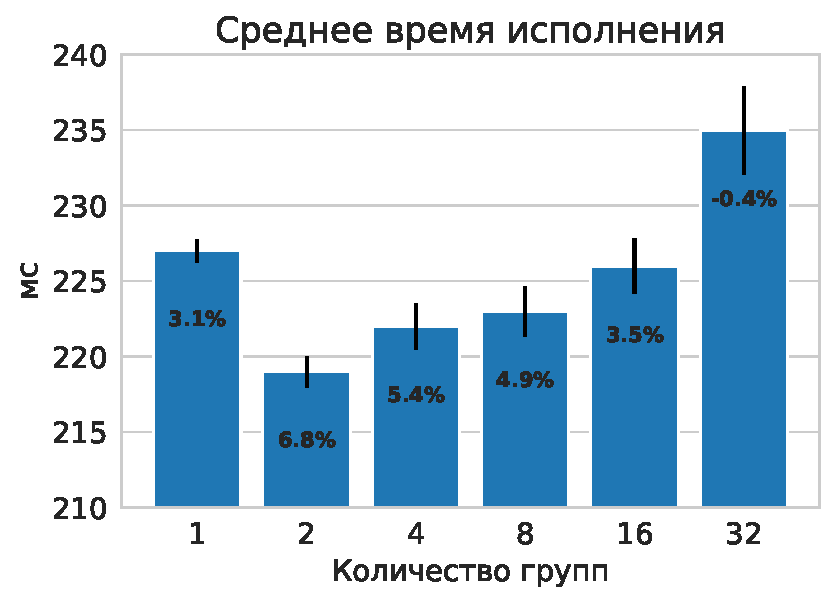
\includegraphics[width=\linewidth]{exp_dispatch_groups.pdf}
    \end{subfigure}
    \hfill
    \begin{subfigure}[t]{.5\textwidth}
    \centering
    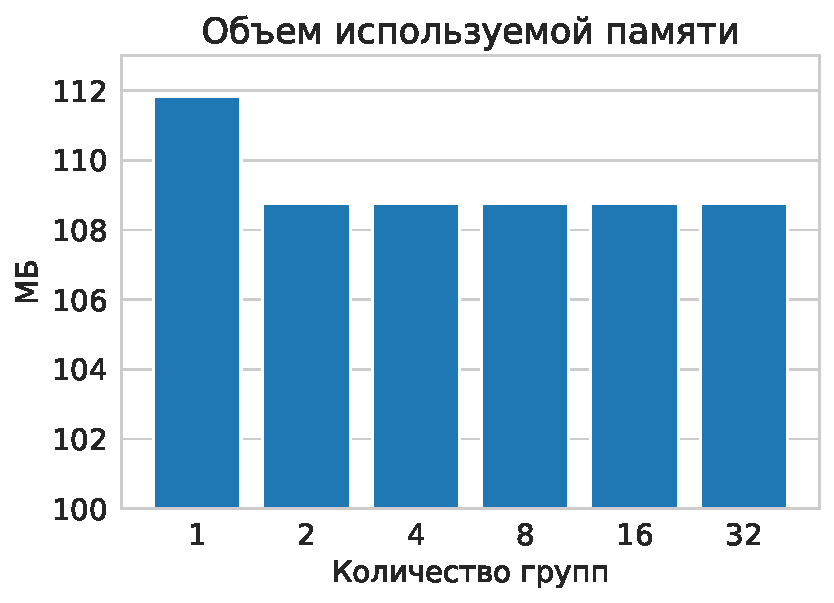
\includegraphics[width=\linewidth]{exp_dispatch_groups_mem.pdf}
    \end{subfigure}
    \begin{subfigure}[t]{.5\textwidth}
    \centering
    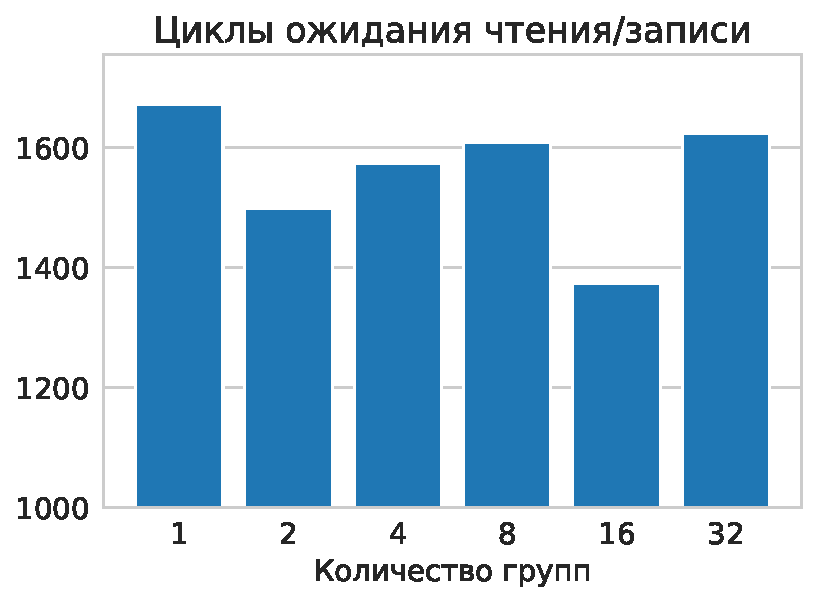
\includegraphics[width=\linewidth]{exp_dispatch_stall.pdf}
    \end{subfigure}
    \hfill
    \begin{subfigure}[t]{.5\textwidth}
    \centering
    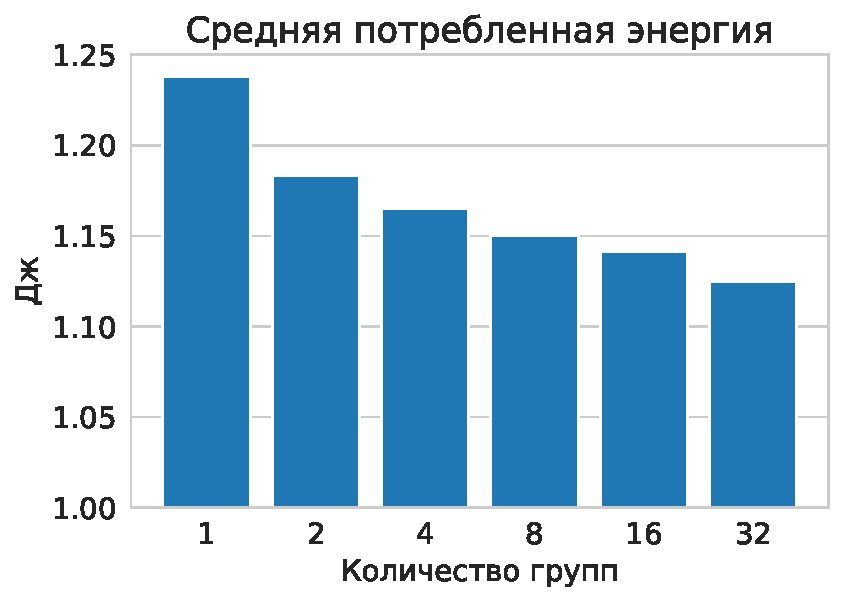
\includegraphics[width=\linewidth]{exp_dispatch_energy.pdf}
    \end{subfigure}
    \captionof{figure}{Столбчатые диаграммы с результатами применения предложенного метода к сети ResNeXt}
    \label{fig:exp_dispatch_groups}
\end{table}
